%-------------------------------------------------------------------------
% corriges-ds-info-S1-ds.tex
%-------------------------------------------------------------------------

%-------------------------------------------------------------------------
\documentclass[11pt,a4paper]{article}
%-------------------------------------------------------------------------

%-------------------------------------------------------------------------
%-------------------------------------------------------------------------
% corriges-ds-info-S1-preambule.tex
%-------------------------------------------------------------------------

%-------------------------------------------------------------------------
\usepackage{calc}
\usepackage[text={16cm,23cm},centering=true,showframe=false]{geometry}
\usepackage{fancybox,fancyvrb,fancyhdr,lastpage,lineno,import}
\usepackage{longtable,multirow}
\usepackage{xcolor,graphics,xmpmulti,pgf,pgfpages,tikz,wrapfig}
\usepackage{colortbl,color}
\usepackage{amsmath,amssymb,amsfonts}
\usepackage{hyperref,multimedia,rotating,framed,pstricks}
\usepackage{listings,index}
%
%---- pdflatex
%\usepackage[T1]{fontenc}
%\usepackage[utf8]{inputenc}
%---- xelatex
\usepackage{fontspec}
%
\usepackage[french]{babel}
\usepackage[french]{nomencl}
\usepackage[framed,hyperref,standard]{ntheorem}
\usepackage{eurosym,pifont}
%-------------------------------------------------------------------------

%-------------------------------------------------------------------------
\lstset
{
language=Python,
basicstyle=\ttfamily,
identifierstyle=\ttfamily,
keywordstyle=\color{blue}\ttfamily,
commentstyle=\color{gray}\ttfamily,
stringstyle=\color{green}\ttfamily,
showstringspaces=false,
extendedchars=true,
numbers=left, 
numberstyle=\color{blue}\tiny,
frame=lines,
linewidth=0.95\textwidth,
xleftmargin=5mm
} 
%-------------------------------------------------------------------------

%-------------------------------------------------------------------------
\pgfdeclareimage[width=3cm,interpolate=true]{logo-enib}{logo-enib}
%-------------------------------------------------------------------------

%-------------------------------------------------------------------------
\pagestyle{fancy}
\fancyhead{}
\fancyhead[L]{\hspace*{-3em}\begin{minipage}{3cm}\pgfuseimage{logo-enib}\end{minipage}}
\fancyhead[C]{Informatique S1}
\fancyhead[R]{\thepage/\pageref{LastPage}}
\fancyfoot{}
\fancyfoot[L]{}
\fancyfoot[C]{}
\fancyfoot[R]{}
\setlength{\headheight}{80pt}
\setlength{\footskip}{38pt}
\renewcommand{\headrulewidth}{0pt}
\renewcommand{\footrulewidth}{0pt}
%-------------------------------------------------------------------------


%-------------------------------------------------------------------------
\def\entete{\noindent\begin{tabular}{|l|l|l|l|} 
\hline 
 & & & \\ 
\makebox[4.55cm][l]{\bsc{Nom :}} & \makebox[4.5cm][l]{\bsc{Prénom :}} & \makebox[2.5cm][l]{\bsc{Groupe :}} & \makebox[2.75cm][l]{\bsc{Question :}} \\[1mm] 
\hline 
\end{tabular}\\[1mm]
{\footnotesize \textsc{Durée : 15'\hfill Documents, calculettes, téléphones et ordinateurs interdits}}}

\def\notes{\begin{tabular}{|c|c|c|c|}  
\hline 
\makebox[0.5cm]{3} & \makebox[0.5cm]{2} & \makebox[0.5cm]{1} & \makebox[0.5cm]{0} \\  
\hline
\end{tabular}  
} 

\def\autoevaluation{$$\begin{tabular}{|c|c|c|}
\hline
\multicolumn{3}{|c|}{\textbf{Auto-évaluation}} \\
\hline
\textbf{M} & \textbf{V} & \textbf{R} \\
Méthode(s) & Vérification(s) & Résultat(s) \\
\notes & \notes & \notes \\[1mm]
\hline
\end{tabular}$$ $$ $$}

\def\reponse{\mbox{}\hfill \fbox{\huge Réponse page suivante}}
%-------------------------------------------------------------------------

%-------------------------------------------------------------------------
\tikzset{
xmin/.store in=\xmin, xmin/.default=-3, xmin=-3,
xmax/.store in=\xmax, xmax/.default=3,  xmax=3,
ymin/.store in=\ymin, ymin/.default=-3, ymin=-3,
ymax/.store in=\ymax, ymax/.default=3,  ymax=3,
}

\newcommand{\grille}{\draw[color=lightgray] (\xmin,\ymin) grid (\xmax,\ymax);}

\newcommand{\axes}{
	\draw[->] (\xmin,0) -- (\xmax,0);
	\draw[->] (0,\ymin) -- (0,\ymax);
}

\newcommand{\fenetre}{\clip (\xmin,\ymin) rectangle (\xmax,\ymax);}
%-------------------------------------------------------------------------

%-------------------------------------------------------------------------
\def\ga{\textsc{ga}}   
\def\bu{\textsc{bu}} 
\def\zo{\textsc{zo}} 
\def\meu{\textsc{meu}} 
%-------------------------------------------------------------------------


%-------------------------------------------------------------------------
\input{sigle}
%-------------------------------------------------------------------------

\graphicspath{{../../../fig/}}



%-------------------------------------------------------------------------

%-------------------------------------------------------------------------
\begin{document}
%-------------------------------------------------------------------------
%$$\mbox{\Large \textbf{DS : algorithmique}}$$

%-------------------------------------------------------------------------
\section{Boucle simple}
%-------------------------------------------------------------------------

{\footnotesize
\begin{lstlisting}
def integration(f,a,b,n) :
    """
    s = integration(f,a,b,n)
    intégrale de la fonction f
    sur [a,b] par la méthode des
    n rectangles
    
    >>> integration(cos,0.,pi,10000)
    4.307866381890461e-16
    >>> integration(cos,-pi/2,pi/2,10000)
    2.000000008224676
    >>> integration(sin,0.,pi,10000)
    2.000000008224676
    >>> integration(exp,0.,1.,10000)
    1.7182818277430947
    >>> integration(log,1.,2.,100)
    0.38629644443195715
    >>> integration(lambda x: 3,1.,2.,10)
    3.0
    >>> integration(lambda x: 3,2.,1.,10)
    -3.0
    >>> integration(lambda x: x,-1.,1.,10)
    8.881784197001253e-17
    >>> integration(lambda x: x*x,-1.,1.,100)
    0.6666000000000001
    >>> integration(lambda x: x**3,0.,1.,100)
    0.24998750000000006
    """
    assert type(a) is float
    assert type(b) is float
    assert type(n) is int and n > 0
    
    s = 0
    d = (b-a)/n
    for i in range(n) :
        s = s + f(a + d/2 + i*d)
    s = s*d
    
    return s
\end{lstlisting}
}
%-------------------------------------------------------------------------
\section{Appels récursifs}
%-------------------------------------------------------------------------

\noindent
\framebox[7.5cm]{\begin{minipage}[t]{7cm}\footnotesize
\begin{enumerate}
\item \texttt{>{>}> f(1,0,100)}
\end{enumerate}
$$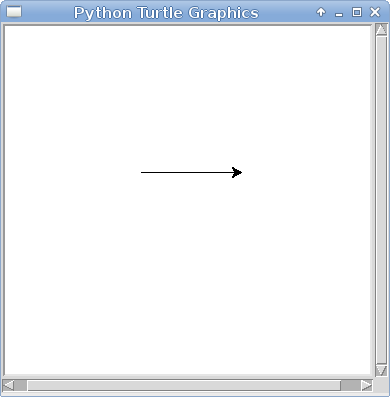
\includegraphics[width=6cm]{f-1-0-100.png}$$
\end{minipage}}
\hfill
\framebox[7.5cm]{\begin{minipage}[t]{7cm}\footnotesize
\begin{enumerate}\setcounter{enumi}{1}
\item \texttt{>{>}> f(1,1,100)}
\end{enumerate}
$$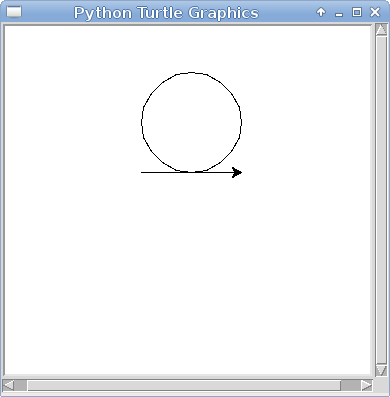
\includegraphics[width=6cm]{f-1-1-100.png}$$
\end{minipage}}
\vspace*{2mm}

\noindent
\framebox[7.5cm]{\begin{minipage}[t]{7cm}\footnotesize
\begin{enumerate}\setcounter{enumi}{2}
\item \texttt{>{>}> f(1,2,100)}
\end{enumerate}
$$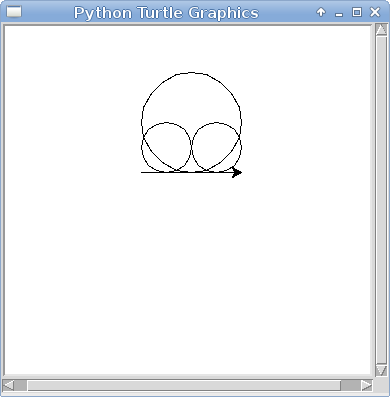
\includegraphics[width=6cm]{f-1-2-100.png}$$
\end{minipage}}
\hfill
\framebox[7.5cm]{\begin{minipage}[t]{7cm}\footnotesize
\begin{enumerate}\setcounter{enumi}{3}
\item \texttt{>{>}> f(2,2,100)}
\end{enumerate}
$$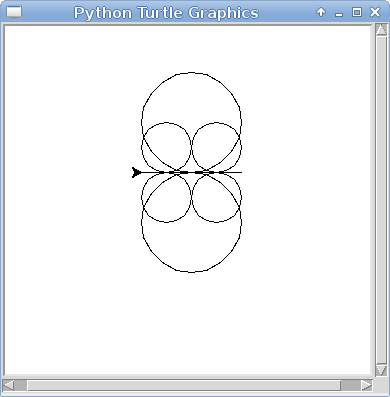
\includegraphics[width=6cm]{f-2-2-100.png}$$
\end{minipage}}
\vspace*{2mm}

\noindent
\framebox[7.5cm]{\begin{minipage}[t]{7cm}\footnotesize
\begin{enumerate}\setcounter{enumi}{4}
\item \texttt{>{>}> f(3,2,100)}
\end{enumerate}
$$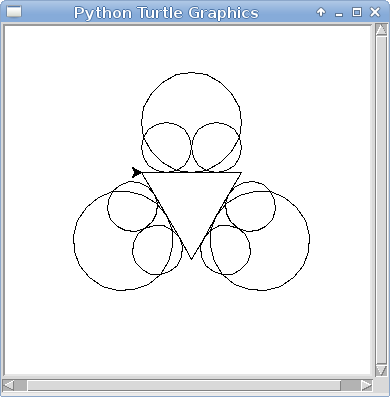
\includegraphics[width=6cm]{f-3-2-100.png}$$
\end{minipage}}
\hfill
\framebox[7.5cm]{\begin{minipage}[t]{7cm}\footnotesize
\begin{enumerate}\setcounter{enumi}{5}
\item \texttt{>{>}> f(4,3,100)}
\end{enumerate}
$$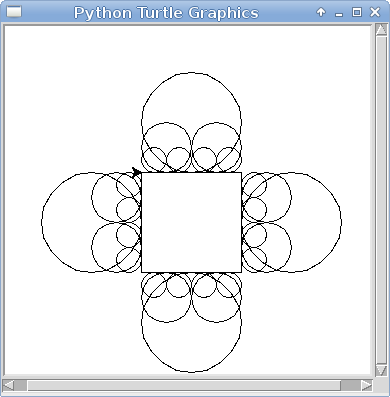
\includegraphics[width=6cm]{f-4-3-100.png}$$
\end{minipage}}
\vspace*{2mm}


%-------------------------------------------------------------------------
\section{Liste de listes}
%-------------------------------------------------------------------------


\footnotesize

\begin{lstlisting}
def listeCarree(t) :
	"""
	ok = listeCarree(t)
	True si t est une liste de n listes de n éléments 
	chacune, False sinon.
	
	>>> listeCarree([])
	True
	>>> listeCarree([[1]])
	True
	>>> listeCarree([[1],[2]])
	False
	>>> listeCarree([[1,7],[2,-3]])
	True
	>>> listeCarree([[2,1,8],[6,0,3]])
	False
	>>> listeCarree([[2,1,8],[6,0,3],[7,5,4]])
	True
	>>> listeCarree([[2,1,8],[6,0,3],[7]])
	False
	"""
    if type(t) is not list : 
        return False
    n = len(t)
    for e in t :
        if not (type(e) is list) :
            return False
        if len(e) != n :
            return False
            
    return True
\end{lstlisting}

\begin{lstlisting}
def appartient(e,t) :
	"""
	ok = appartient(e,t)
	True si e appartient à la liste carrée t,
	False sinon
	
	>>> t = [[2,1,8],[6,0,3],[7,5,4]]
	>>> appartient(5,t)
	True
	>>> appartient(9,t)
	False
	"""
    assert listeCarree(t)
    
    for elem in t :
        if e in elem :return True
    
    return False
\end{lstlisting}

\newpage
\begin{lstlisting}
def Taquin(t) :
	"""
	ok = Taquin(t)
	True si la liste carrée t est un jeu de Taquin,
	False sinon.
	
	>>> Taquin([[0,1,2]])
	False
	>>> Taquin([[3,1],[0,2]])
	True
	>>> Taquin([[2,1,8],[6,0,3],[7,5,4]])
	True
	>>> Taquin([[2,1,8],[6,0,3],[7,5,0]])
	False
	"""
    if not listeCarree(t) :
        return False
    n = len(t)
    for i in range(n*n) :
        if not appartient(i,t) :
            return False
            
    return True
\end{lstlisting}

\begin{lstlisting}
def carreauVide(jeu) :
    """
    (i,j) = carreauVide(jeu)
    position du carreau vide dans la
    configuration jeu d'un jeu de Taquin
    
    >>> carreauVide([[3,1],[0,2]])
    (1, 0)
    >>> carreauVide([[2,1,8],[6,0,3],[7,5,4]])
    (1, 1)
    """
    assert Taquin(jeu)

    n = len(jeu)
    ok = False
    i = 0
    while i < n and not ok :
       if 0 in jeu[i] :
           j = 0
           while j < n and not ok :
               if jeu[i][j] == 0 : ok = True
               else : j = j + 1
       else : i = i + 1
    return (i,j)
\end{lstlisting}

\begin{lstlisting}
def jouerTaquin(jeu) :
    """
    suivants = jouerTaquin(jeu)
    liste des configurations de Taquin
    immédiatement accessibles à partir
    de la configuration initiale jeu
    
    >>> jeu  = [[3,1],[0,2]]
    >>> jouerTaquin(jeu)
    [[[0, 1], [3, 2]], [[3, 1], [2, 0]]]
    >>> jeu  = [[2,1,8],[6,0,3],[7,5,4]]
    >>> jouerTaquin(jeu)
    [[[2, 0, 8], [6, 1, 3], [7, 5, 4]], [[2, 1, 8], [6, 5, 3], [7, 0, 4]], [[2, 1, 8], [0, 6, 3], [7, 5, 4]], [[2, 1, 8], [6, 3, 0], [7, 5, 4]]]
    """
    assert Taquin(jeu)
    
    n = len(jeu)
    (i0,j0) = carreauVide(jeu)
    suivants = []

    (i1,j1) = (max(0,i0-1),j0)
    jeu1 = permuterVide(jeu,(i0,j0),(i1,j1))
    if jeu1 != jeu :
        suivants.append(jeu1)

    (i1,j1) = (min(i0+1,n-1),j0)
    jeu1 = permuterVide(jeu,(i0,j0),(i1,j1))
    if jeu1 != jeu :
        suivants.append(jeu1)

    (i1,j1) = (i0,max(0,j0-1))
    jeu1 = permuterVide(jeu,(i0,j0),(i1,j1))
    if jeu1 != jeu :
        suivants.append(jeu1)

    (i1,j1) = (i0,min(j0+1,n-1))
    jeu1 = permuterVide(jeu,(i0,j0),(i1,j1))
    if jeu1 != jeu :
        suivants.append(jeu1)

    return suivants
\end{lstlisting}

\begin{lstlisting}
def permuterVide(jeu,pos1,pos2) :
    """
    jeu1 = permuterVide(jeu,pos1,pos2)
    nouvelle configuration de Taquin obtenue
    en déplaçant le carreau vide
    de la position pos1 à la position pos2
    dans la configuration initiale jeu
    
    >>> permuterVide([[3,1],[0,2]],(1,0),(0,0))
    [[0, 1], [3, 2]]
    >>> permuterVide([[3,1],[0,2]],(1,0),(1,1))
    [[3, 1], [2, 0]]
    """
    assert Taquin(jeu)
    assert type(pos1) is tuple and len(pos1) == 2
    assert type(pos2) is tuple and len(pos2) == 2

    n = len(jeu)
    jeu1 = []
    for i in range(n) :
        jeu1.append([])
        for j in range(n) :
            jeu1[i].append(jeu[i][j])            
    jeu1[pos1[0]][pos1[1]], jeu1[pos2[0]][pos2[1]] = jeu1[pos2[0]][pos2[1]], jeu1[pos1[0]][pos1[1]]
    return jeu1
\end{lstlisting}


%-------------------------------------------------------------------------
\end{document}
%-------------------------------------------------------------------------
